
\documentclass[12pt]{amsart}
\usepackage{geometry} % see geometry.pdf on how to lay out the page. There's lots.
\geometry{a4paper} % or letter or a5paper or ... etc
% \geometry{landscape} % rotated page geometry
\usepackage{caption}
\usepackage{graphicx}
\usepackage[backend=bibtex,style=verbose-trad2]{biblatex}
\bibliography{biblio}
% See the ``Article customise'' template for come common customisations

\title{LTV prediction using probabilistic models}
\author{}
\date{} % delete this line to display the current date

%%% BEGIN DOCUMENT
\begin{document}

\maketitle
\tableofcontents

\section{Introduction}

In this project we want to perform an estimation of customer life-time value (LTV) as a case of a Customer-Base Analysis using what literature in this domain calls probabilistic models (which is in reality no other thing that using Bayesian approach),using data from the company where we work .

This work will be divided in the following parts: First discussion Customer-Basis Analysis and possibles scenarios and characterization of our scenario, second description of the model we will use (assumptions, ...), third discussion about implementation and finally presentation of results and accuracy measurement.

We found that this would make a proper project for a "Bayesian Statistics" course, as it is in between a Data-oriented and an Application-oriented project type.

\section{Customer Basis Analysis:}

Customer Basis Analysis is a concept that is being more and more critical as Companies have access (or generate) to more customer's transaction data (increase in complexity and volume). This avaibility of these datasets has lead to a general change to transaction based strategies to more customer-centric strategies. In other words, the first strategies lead typically to descriptive analysis (for example summary statistic like rates, average number of subscriptions ...), while the more customer-centric approach is more focused on analysis on activities that are more predictive, i.e. activities and facts that by past information (found in those databases) a forecast is made. This is why a Bayesian Probabilistic approach can be convenient.

\subsection{Probabilistic models for Customer Basis Analysis:}
\hfill\\

How can we model this analysis with Probabilistic Models ? As usual in this situations, problem will be modeled in a way that observed behavior has underlying a random process, thus a past behavior is not a true mirror of future actions. With this interpretation, the past, and the "future" are function of latent characteristics denoted by $\theta$ .

While this approach may not be new (in other fields), the novelty resides in the fact that classically for Customer Basis Analysis, the approaches have been regression-like (which also happened in the company we work) and the use of probabilistic approaches is relatively new.

\subsection{Possible scenarios:}
\hfill\\

Commonly in literature we will find the following classification for scenarios in Customer-Base Analysis :
\hfill\\
\textbf{By Opportunities of Transactions:}
\hfill\\
It can be discrete and continuous.
\hfill\\
\textbf{By Relation with the Customer:}
\hfill\\
The key distinction between contractual and noncontractual is that in contractual scenario, you observe when a customer leaves, while in a noncontractual scenario, customer departure is unobservable and therefore must be inferred. For example in a contractual scenario, a user might pay for a service only when needed, so that if during a long time this user didn't made any transaction either it should be considered that is not any more a client or it's just a hiatus, we don't know it directly.


\begin{figure}[h!]
  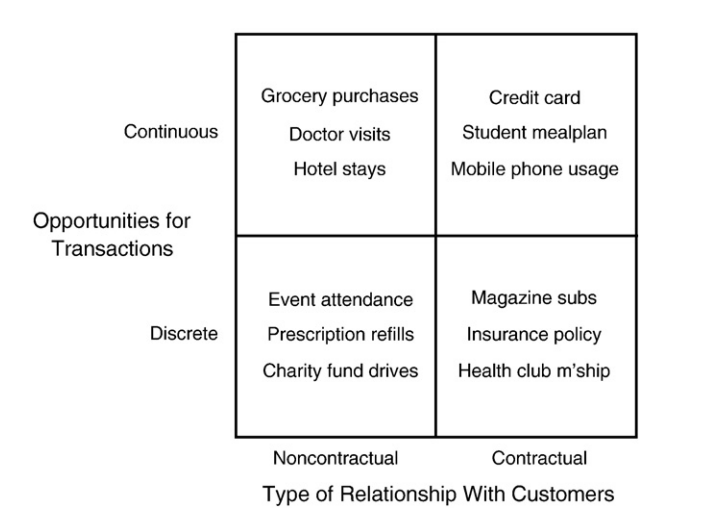
\includegraphics[scale = 0.75]{CustomerRelation.png}
  \caption{Examples for the different scenarios. From \cite{fader09} }
  \label{fig:Relation}
\end{figure}

Correctly knowing in which scenario our problem is in matters, especially while selecting a model.

The company in which we work, has a few subscription based websites, where users are subscrived in order to have access to contents and services. After each cycle (30 days) the user is automatically rebilled and in order to drop out, the user should cancel. As a consequence this scenario corresponds to a contractual scenario where transactions are done periodically.

In concrete we will work with data from a concrete product.

\subsection{Our case : Model LTV prediction}
\hfill\\

For the scope of this project, we will model a the Customer Life Time Value (or LTV) as a particular case of Customer Basis Analysis, using Bayesian Probabilistic model.

In marketing, customer lifetime value (CLV or often CLTV), lifetime customer value (LCV), or life-time value (LTV) is a prediction of the net profit attributed to the entire future relationship with a customer. The prediction model can have varying levels of sophistication and accuracy, ranging from a crude heuristic to the use of complex predictive analytics techniques.

For this we will first implement the proposed model for Customer Retention Prediction described in \cite{fader07}, on a dataset of one of the products of the company.

\section{Dataset description}

 Our case is of a Discrete Contractual scenario (as we see in \ref{fig:Relation}) , with a 30 days period cycle of rebill. The users can cancel their relation with the company at any time.
 The data we use has been collected from July the15th and July the 15th, and it is composed of number of clients that rebills after each cycle, for one of the company products.
 We have added two additional columns that may be useful , the number of clients as a percentage and the number of users that cancels during each cycle.

 \begin{figure}[h!]
  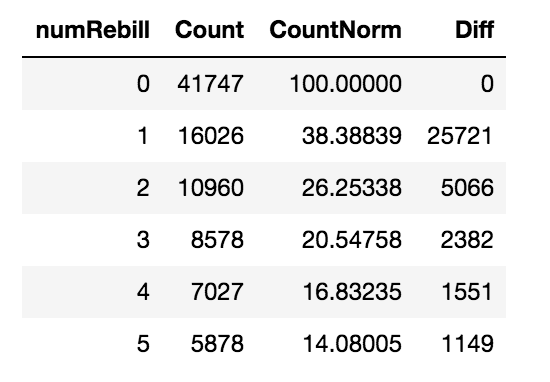
\includegraphics[scale = 0.55]{Data_sample.png}
  \caption{Number of user rebilling at each cycle}
  \label{fig:Data_sample}
\end{figure}

\section{Model  : Shifted Geometrical Beta distribution for retention prediction}
 
 Our first idea to approach this problem was using a Inverse Binomial with a Beta distribution as prior. We first tried this implementation with a MCMC implementation in order to estimate the probability of cancel of the users. But at the end we rejected this model as it just considered the users that cancelled and not the remaining users. Then we found the model presented in \cite{feder07} that also considers the users that doesn't cancels after the observation period.
 
 The model we want to test is also based in using a negative binomial distribution (more precisely a geometric distribution as the failure number $r$ is set to 1), with some other considerations that enables to consider the surviving users. Let's see the model in more detail. 
 
 \subsection{Model Assumptions}
 \hfill\\
 
 First the assumptions for the model :
 \begin{itemize}
  \item At the end of each cylce, the user renews its subscription or cancels with some probability
  \item That probability remains constant
  \item There is the assumption of heterogeneity between clients
\end{itemize}
 
 Those assumptions are translated in the following probabilities : 
 \hfill\\
 
 The probability of duration for a given user( we will call it retention function), in terms of counts of rebills (success) before cancel the contract (failure), thus a classical Negative Binomial (with $r$ =1, also called Geometric)
 \begin{equation} \label{eq1}
 P(T=t | \theta) = \theta (1-\theta)^{t-1}
 \end{equation}
 \hfill\\
 
 The other is the probability of remaining as client in for a given cycle (survival function), which is a Negative Binomial with $r$=0 :
  \begin{equation} \label{eq2}
S(t | \theta) = (1-\theta)^t
 \end{equation}
 \hfill\\
 
  Where $T$ is the number of cycles that the user has rebilled (the number of counts), and $\theta$ the probability of cancel.
  
  So in this model, the parameter that is not directly measurable and has to be estimated is $\theta$
. 
 \subsection{Prior and Likelihood}
 \hfill\\
 
For this setting it is not a bad assumption to consider as a prior distribution for $\theta$ a Beta distribution, as it can be fitted to our data, with a proper choice of $\alpha$ and $\beta$ parameters. 

Prior Distribution :

\begin{equation} \label{eq3}
f(\theta; \alpha, \beta) = \frac{\theta^{\alpha-1}(1-\theta)^{\beta-1}}{B(\alpha,\beta)}
\end{equation}

As for the Likelihood function, we should not forget what we want to model. In a classic scenario of counting successes/failures, we would only take into consideration the retention probability part i.e. the users that cancels after a number of rebills, ( thus with a Negative Binomial distribution the problem ). In our case, we want to model either the behavior of the users that cancelled after some cycles and the users still in contract (the idea on doing this approach is that with data of few cycles we can predict behavior of the following cycles). That's the reason a survival (equation \ref{eq2}) function is considered.

Let's assume that we have data for a limited number of cycles, that we call $T_max$. Assuming independence between users, we will have as a liklihood distribution : 

\begin{equation} \label{eq4}
\prod_{t=1}^{T_{max}}P(T=t | \theta)^{n_t}S(T_{max} | \theta)^{N-\sum_{t=1}^{T_{max}}n_t}
\end{equation}

where :

 \begin{itemize}
  \item  $n_t$ is the number of users that cancels on cycle $t$
  \item  $N$ is the number of total subscriptions (i.e. users that made transaction rebill 0)
  \item  $T_{max}$ is the maximum number of cycles
\end{itemize}
 \hfill\\
 
Note that this equation has two distinguishable parts : 
The first term, 
$
\prod_{t=1}^{T_{max}}P(T=t | \theta)^{n_t}
$
models the probability of users that had cancelled before $T_{max}$ cycle and the second term $S(T_{max} | \theta)^{N-\sum_{t=1}^{T_{max}}n_t}$  the probability of the users still "alive". So we consider a term that is not in a classical Negative Binomial scenario.

As this likelihood term doesn't correspond exactly to any standard distribution, we opted for a Posterior Maximization strategy to estimate the parameter.

For this the approach that is used at \cite{feder07} is to compute the likelihood function as a function of $\alpha$ and $\beta$ parameters by averaging the likelihood with the prior (thus in reality computing the posterior predictive) and maximize for $\alpha$ and $\beta$. 

The derivations to obtain such expressions (adapted from \cite{feder07} ) :

For the retention part : 

\begin{align*}
P(T=t | \alpha,\beta) &= \int_0^1 P(T=t | \Theta = \theta)f(\theta ;  \alpha,\beta) d\theta \\ &= 
\int_0^1 \theta (1-\theta)^{t-1}  \frac{\theta^{\alpha-1}(1-\theta)^{\beta-1}}{B(\alpha,\beta)} d\theta \\
&=\frac{1}{B(\alpha,\beta)}  \int_0^1 \theta^{\alpha}(1-\theta)^{\beta+t-2}d\theta \\
&= \frac{B(\alpha+1,\beta+t-1)}{\alpha,\beta}
\end{align*} 

For the survival part : 

\begin{align*}
S(t | \alpha,\beta) &= \int_0^1 S(t | \Theta = \theta)f(\theta ;  \alpha,\beta) d\theta \\ &= 
\int_0^1  (1-\theta)^{t}  \frac{\theta^{\alpha-1}(1-\theta)^{\beta-1}}{B(\alpha,\beta)} d\theta \\
&=\frac{1}{B(\alpha,\beta)}  \int_0^1 \theta^{\alpha-1}(1-\theta)^{\beta+t-1}d\theta \\
&= \frac{B(\alpha,\beta+t)}{\alpha,\beta}
\end{align*} 

The retention part has been implemented in a recursive way, using the expression proposed in the article: 

First we should note that:
$$
\frac{\gamma(x+1)}{\gamma(x)}=x
$$

$$
B(\alpha,\gamma)=\frac{\gamma(\alpha)\gamma(\beta)}{\gamma(\alpha + \beta)}
$$

The general recursive expression : 

$$
P(T = t | \alpha,\beta) = \frac{P(T = t | \alpha,\beta)}{P(T = t -1| \alpha,\beta)}P(T = t-1 | \alpha,\beta)
$$

First we have to compute the initial expression in which we use the above expressions of the Gamma function and the definition of Beta function in terms of Gamma functiond : 

$$
P(T = 1 | \alpha,\beta) =\frac{B(\alpha+1,\beta)}{B(\alpha,\beta)} = \frac{\gamma(\alpha + 1)/\gamma(\alpha)}{\gamma(\alpha + \beta +1)/\gamma(\alpha + \beta)} = \frac{\alpha}{\alpha + \beta} 
$$

Then we can compute the first term of the recursive expression :

\begin{align*}
 \frac{P(T = t | \alpha,\beta)}{P(T = t -1| \alpha,\beta)} &= \frac{B(\alpha+1,\beta+t-1)}{B(\alpha+1,\beta+t-2)} \\�&=  \frac{\gamma(\beta + t - 1)/\gamma(\beta + t -2)}{\gamma(\alpha + \beta +t)/\gamma(\alpha + \beta + t -1)} \\ &= \frac{\beta+t-2}{\alpha+\beta+t-1} 
\end{align*}

So at the end the recursive expression  is : 

\begin{equation} \label{eq5}
P(T=t | \alpha, \beta) = 
\left\{
	\begin{array}{ll}
		\frac{\alpha}{\alpha + \beta}  & \mbox{if } t =1 \\
		\frac{\beta + t -2}{\alpha + \beta + t -1}P(T=t|\alpha,\beta) & \mbox{if } t > 1
	\end{array}
\right.
\end{equation}

\subsection{Maximum Likelihood}
 

\begin{thebibliography}{9}
    
    \bibitem{feder07}
    Peter S. Fader and Bruce G. S. Hardie
    \textit{ How To Project Customer
Retention},
    2007.
    
        \bibitem{feder09}
    Peter S. Fader and Bruce G. S. Hardie
    \textit{ Probability Models for Customer-Base Analysis},
    2009.
    
\end{thebibliography}
\end{document}